\section{BPMN example output}\label{app-output}
The following output shows the output of the implemented software when giving the example \ref{fig:example-process} BPMN as input.
\begin{lstlisting}[breaklines=true, language=json]
[
{
	"title": "No two consecutive Tasks should be executed by the same resource",
	"description": "Two task that are executed one after the other can be merged if they have the same enitity executing the Task. In case of User tasks this means the same usergroup is executing this task. Automated Tasks that follow each other should also always be merged to minimize flownodes.",
	"details": "The Returned Effected Elements represent a list of tasks that can be merged with its direct successor.In case that three or more tasks can be merged, this algorithm will return every Task that can be mergedwith its successor on its own. Therefore if \"task1\" , \"task2\" and \"task3\" can be merged all together, this algorithm will \"task2\" and \"task3\" as effected elements",
	"effectedElements": [
	{
		"id": "CancelRelatedWebIdent",
		"name": "Cancel Related Identification Process Instances",
		"type": "Task"
	},
	{
		"id": "ReserveMsisdn",
		"name": "Reserve phone number",
		"type": "Task"
	},
	{
		"id": "BookAutoTopups",
		"name": "Book further multi options",
		"type": "Task"
	},
	{
		"id": "ServiceTask_0p0tajd",
		"name": "Start Belated Porting",
		"type": "Task"
	},
	{
		"id": "ServiceTask_0e2r82f",
		"name": "Create Porting-Info History Entry",
		"type": "Task"
	},
	{
		"id": "BookSingleTopups",
		"name": "Book further single options",
		"type": "Task"
	}
	]
},
{
	"title": "No manual Tasks are allowed",
	"description": "Manual Tasks should not be part of an executable BPMN diagram",
	"details": "The Returned Effected Elements represent a list of manual tasks in the given diagram",
	"effectedElements": [
	{
		"id": "data_to_warehouse",
		"name": "store data into datastore",
		"type": "Task"
	}
	]
},
{
	"title": "Event based gateways instead of a parallel gateway followed by exclusive gateways",
	"description": "Event based gateways should be used instead of a parallel gateway followed by one or more exclusive gateways",
	"details": "This Rule applied whenever a parallel gateways is followed by one or more exclusive gateways. The returned Effected Elements are a list of parallel gateways that are followed by one or more exclusive gateways in the given diagram",
	"effectedElements": [
	{
		"id": "ParallelGateway_0crudor",
		"name": null,
		"type": "Gateway"
	}
	]
},
{
	"title": "Apply naming conventions",
	"description": "One aspect of naming convention is the length of labels, this rule scanns the bpmn for rlements with long labels (> 5 words)",
	"details": "The returned effected elements are all elements with a label that has more than 5 words",
	"effectedElements": [
	{
		"id": "ServiceTask_DefaultDocWorkflowPostAwaitConfirmation",
		"name": "validate address, validate payment and create contract",
		"type": "Task"
	},
	{
		"id": "DecideIdAndCsProcess",
		"name": "Decide non default doc flow and idnetification Process",
		"type": "Task"
	},
	{
		"id": "save_member_for_riskident",
		"name": "save new member in backend service",
		"type": "Task"
	}
	]
}
]
\end{lstlisting}
\section{Case Study - Implemented Aprovements}\label{BPMN-improvements}
The following section shows the improvement steps done in section \ref{improvements}.

\newgeometry{top=0.1cm}
\begin{figure}
	\centering
	\includegraphics[width=1.7\columnwidth, angle=90]{graphics/register-customer/2-registercustomer-renaming-bpmn.pdf}
	\caption{Adapted customer registrations process, after renaming} 
	\label{fig:process-renaming} 
\end{figure}
\begin{figure}[H]
	\centering
	\includegraphics[width=1.7\columnwidth, angle=90]{graphics/register-customer/3-registercustomer-manual-bpmn.pdf}
	\caption{Adapted customer registrations process, after changing the manual task to a user task} 
	\label{fig:process-manual} 
\end{figure}

\begin{figure}[H]
	\centering
	\includegraphics[width=1.7\columnwidth, angle=90]{graphics/register-customer/4-registercustomer-merge-bpmn.pdf}
	\caption{Adapted customer registrations process, after merging tasks that are executed by the same resource} 
	\label{fig:process-merge} 
\end{figure}

\begin{figure}[H]
	\centering
	\includegraphics[width=1.7\columnwidth, angle=90]{graphics/register-customer/5-registercustomer-exclusive-bpmn.pdf}
	\caption{Adapted customer registrations process, after changing the combined parallel and exclusive gateways to an inclusive gateway } 
	\label{fig:process-inclusive} 
\end{figure}
\restoregeometry
\section{Case Study - Value Added Analysis}\label{BPMN-vaa}
The following section shows resources needed for the implementation of value added analysis in section \ref{improv-vaa}.

\newgeometry{top=0.1cm}
\begin{figure}[H]
	\centering
	\includegraphics[width=1.7\columnwidth, angle=90]{graphics/register-customer/6-registercustomer-vaa.pdf}
	\caption{Adapted customer registrations process with colored in activities according after value added analysis} 
	\label{fig:process-vaa} 
\end{figure}

\begin{figure}[H]
	\centering
	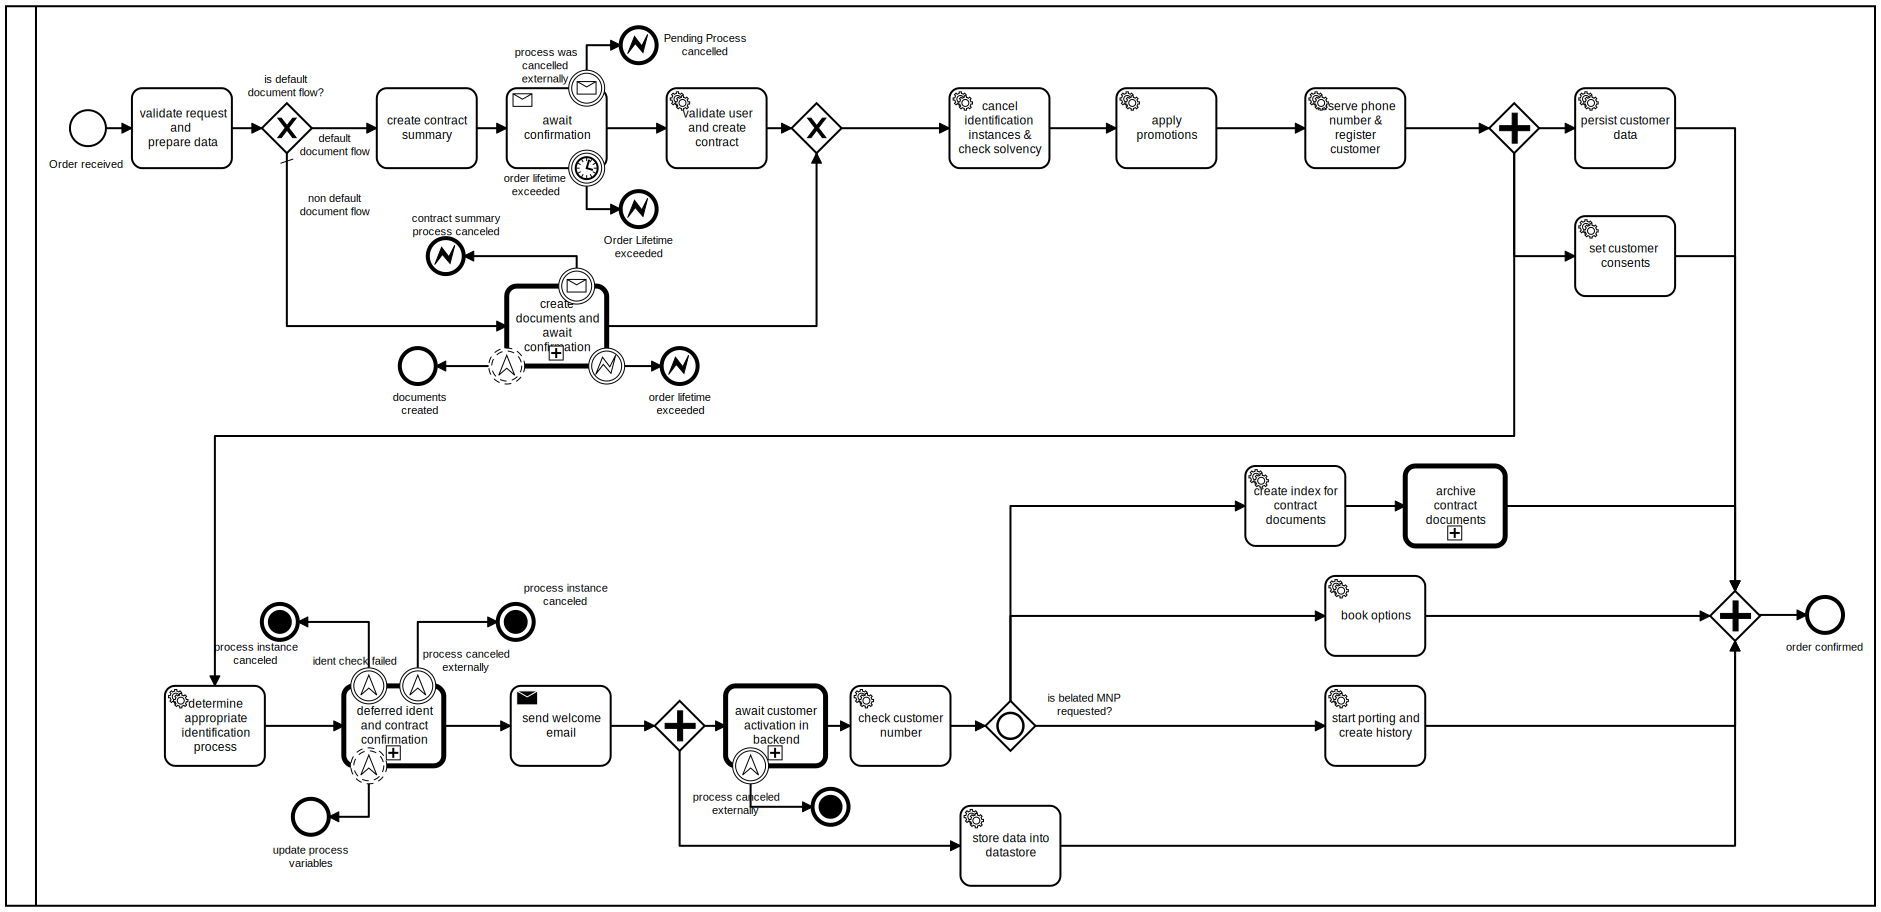
\includegraphics[width=1.7\columnwidth, angle=90]{graphics/register-customer/7-registercustomer-waste-elimination.pdf}
	\caption{Adapted customer registrations process after waste elimination} 
	\label{fig:process-vaa-waste} 
\end{figure}